\chapter{电化学分析}

\begin{introduction}
	\item 电化学的基本概念(掌握)
	\item 电位分析法测定pH值的方法(掌握)
	\item 电位分析法的电极(了解)
	\item 电解和库仑分析法(理解)
	\item 极谱分析法(了解)
	\item 循环伏安法(了解)
\end{introduction}


%设计方案:
%1.定义、概念、原理,做个环境
%2.公式、符号说明环境
%3.步骤、结构、小点:列表
%4.对比:表格

\section{电化学的基本概念}

\begin{definition*}{电池}{}
	是指两个电极被至少一个电解质相所隔开的体系。它是电化学分析法中必不可少的装置。
	
	三要素:电极、电解质、外电路
	
	分类:原电池和电解池
\end{definition*}

%不写nerst方程、原电池表示吗

\begin{definition*}{原电池}{}
	化学能转化成电能的装置。
	

\end{definition*}

\begin{definition*}{电解池}{}
	将电能转化为化学能的装置。
\end{definition*}

不管是原电池还是电解池,发生氧化反应的电极称为阳极,发生还原反应的电极称为阴极;%电位高的为正极,电位低的为负极。


\section{电位分析法}
2、掌握电位分析法测定pH值的方法。了解电位分析法的电极—指示电极(玻璃电极即pH电极、离子选择性电极、生物电极(酶电极和免疫电极等))和参比电极(饱和甘汞电解和银/氯化银电极)。
测量的是电池的电动势(电极电位),根据能斯特方程,把待测物的浓度和电位联系起来。化学电池是原电池。

这一部分所用的化学电池是原电池。

\subsection{理论基础}
能斯特方程
\begin{equation*}
	\varphi=\varphi^{\Theta}+\dfrac{RT}{nF}\lg \dfrac{\Pi a_{ox}}{\Pi a_{red}}
\end{equation*}

$n$为电极反应电子数,$F=96485\mathrm{C/mol}$为法拉第常数,

\subsection{指示电极}
指示电极(indicator electrode)的作用是指示与被测物质的浓度相关的电极电位.


\subsection{参比电极}


\section{电解和库仑分析法}
%3、理解电解和库仑分析法。化学电池是电解池?什么是分解电压?

这一部分所用的化学电池是电解池。

\subsection{电解分析法}
\begin{definition*}{电解分析法}{}
	通过测量电解中沉积于电极表面的沉积物质量进行分析的一类方法。
\end{definition*}

\begin{example}
	现以电解0.5mol/L\ $\ce{H2SO4}$和$\ce{CuSO4}$的混合溶液为例说明电解过程。
	
	\begin{itemize}
		\item 阴极:$\ce{Cu^2+ + 2e- -> Cu}$
		\item 阳极:$\ce{2H2O - 2e- -> O2 + 4H+}$
	\end{itemize}

	可以测量沉积于阴极表面的$\ce{Cu}$的质量,对溶液进行分析,如测量$\ce{Cu^2+}$浓度。
\end{example}

结合标准电极电势和能斯特方程可计算出阴阳极的实际电位$E_{\text{阴}},E_{\text{阳}}$。

\begin{definition*}{理论分解电压}{}
	\begin{equation*}
	E_{\text{分,理}}=E_{\text{阳}}-E_{\text{阴}}
	\end{equation*}
\end{definition*}

但由于iR降(克服电解质溶液的电阻)、过电位(阴阳极的极化现象),使电解发生所需的实际电压要高于$E_{\text{分,理}}$。

\begin{definition*}{(实际)分解电压}{}
	\begin{equation*}
	E_{\text{分}}=E_{\text{分,理}}+iR+\eta_{\text{阳}}-\eta_{\text{阴}}
	\end{equation*}
\end{definition*}

其中
\begin{itemize}
	\item i为电解电流,R为电解回路总电阻;
	\item $\eta_{\text{阳}},\eta_{\text{阴}}$分别是阳极、阴极的超电位,即电极电位与可逆电极电位的差值。
\end{itemize}

注:极化、过电位这里没再深入。

电解分析的主要类别有:
\begin{definition*}{控制电位电解分析}{}
	工作电极的电位控制在某一合适的电位值或某一个小范围内,使被测离子在工作电极上析出,其它离子则留在溶液中,以达到{\heiti 分离和测定}的目的。
\end{definition*}

\begin{example}
	电解1mol/L$\ce{Cu^2+}$和0.01mol/L$\ce{Ag+}$的混合溶液。
	
	\begin{itemize}
		\item $E_{\ce{Cu^2+}}=0.337\mathrm{V}$
		\item $E_{\ce{Ag+}}=0.681\mathrm{V}$,故银先析出
		\item 当$c_{\ce{Ag+}=10^{-6}}\mathrm{mol/L}$时,$E_{\ce{Ag+}}=0.445\mathrm{V}$,铜仍不会析出,故能分离两种离子。
	\end{itemize}
	
	可以测量沉积于阴极表面的$\ce{Cu}$的质量,对溶液进行分析,如测量$\ce{Cu^2+}$浓度。
\end{example}

恒电流电解分析、汞阴极电解分析的例子在课本上,不确定是否考,暂未列入。

\subsection{库仑分析法}
\begin{definition*}{库仑分析法}{}
	通过测量电解中消耗的电量进行分析的一类方法。
\end{definition*}
	
\begin{gather*}
	m=\dfrac{MQ}{nF}\\
	Q=\int i\di{t}
\end{gather*}

其中$m$为析出的物质的量,$M$为该物质的相对量,$n$为电极反应电子数,$Q$为通过的总电荷量。

库仑分析法主要分为:

\begin{itemize}
	\item 控制电位库仑分析:通过库仑计求出电量$Q$,直接参与计算。
	\item 恒电流库仑分析:控制电解电流一定,又称库仑滴定法。
\end{itemize}
%怎么恒电流的还没清楚

\begin{example}
	测$\ce{AsO3^3-}$含量。在$\ce{H2SO4}$介质,$\ce{KBr}$辅助电解质中,
	
	\begin{itemize}
		\item 阴极:$\ce{2H+ + 2e- -> H2 ^ }$
		\item 阳极:$\ce{2Br- - 2e- -> Br2}$
	\end{itemize}

	电解产生$\ce{Br2}$立即氧化$\ce{AsO3^3-}$:
	
	$\ce{AsO3^3- + Br2 + H2O -> AsO4^3- + 2Br- + 2H+}$
	
	恢复了电极反应的物质,所以电动势不变,电流也不变,直到$\ce{AsO3^3-}$耗尽,电流计指针偏转指示终点。此法叫死停终点法。
\end{example}


\section{伏安分析法}
%4、了解极谱、伏安分析法?什么是极限扩散电流?什么是半波电位?

伏安分析法(voltammetry)是指以被分析溶液中电极的电压-电流行为为基础的一类电化学分析方法。与电位分析法不同,伏安分析法是在一定的电位下对体系电流的测量。

\subsection{极谱分析法}





\begin{definition*}{极限扩散电流}{}
	通过测量电解中沉积于电极表面的沉积物质量进行分析的一类方法。
\end{definition*}

\begin{definition*}{半波电位}{}
	通过测量电解中沉积于电极表面的沉积物质量进行分析的一类方法。
\end{definition*}


\subsection{循环伏安法}
如果以三角波电位进行扫描,所获得的电流响应与电位信号的关系称为循环伏安扫描曲线。
\begin{figure}
	\centering
	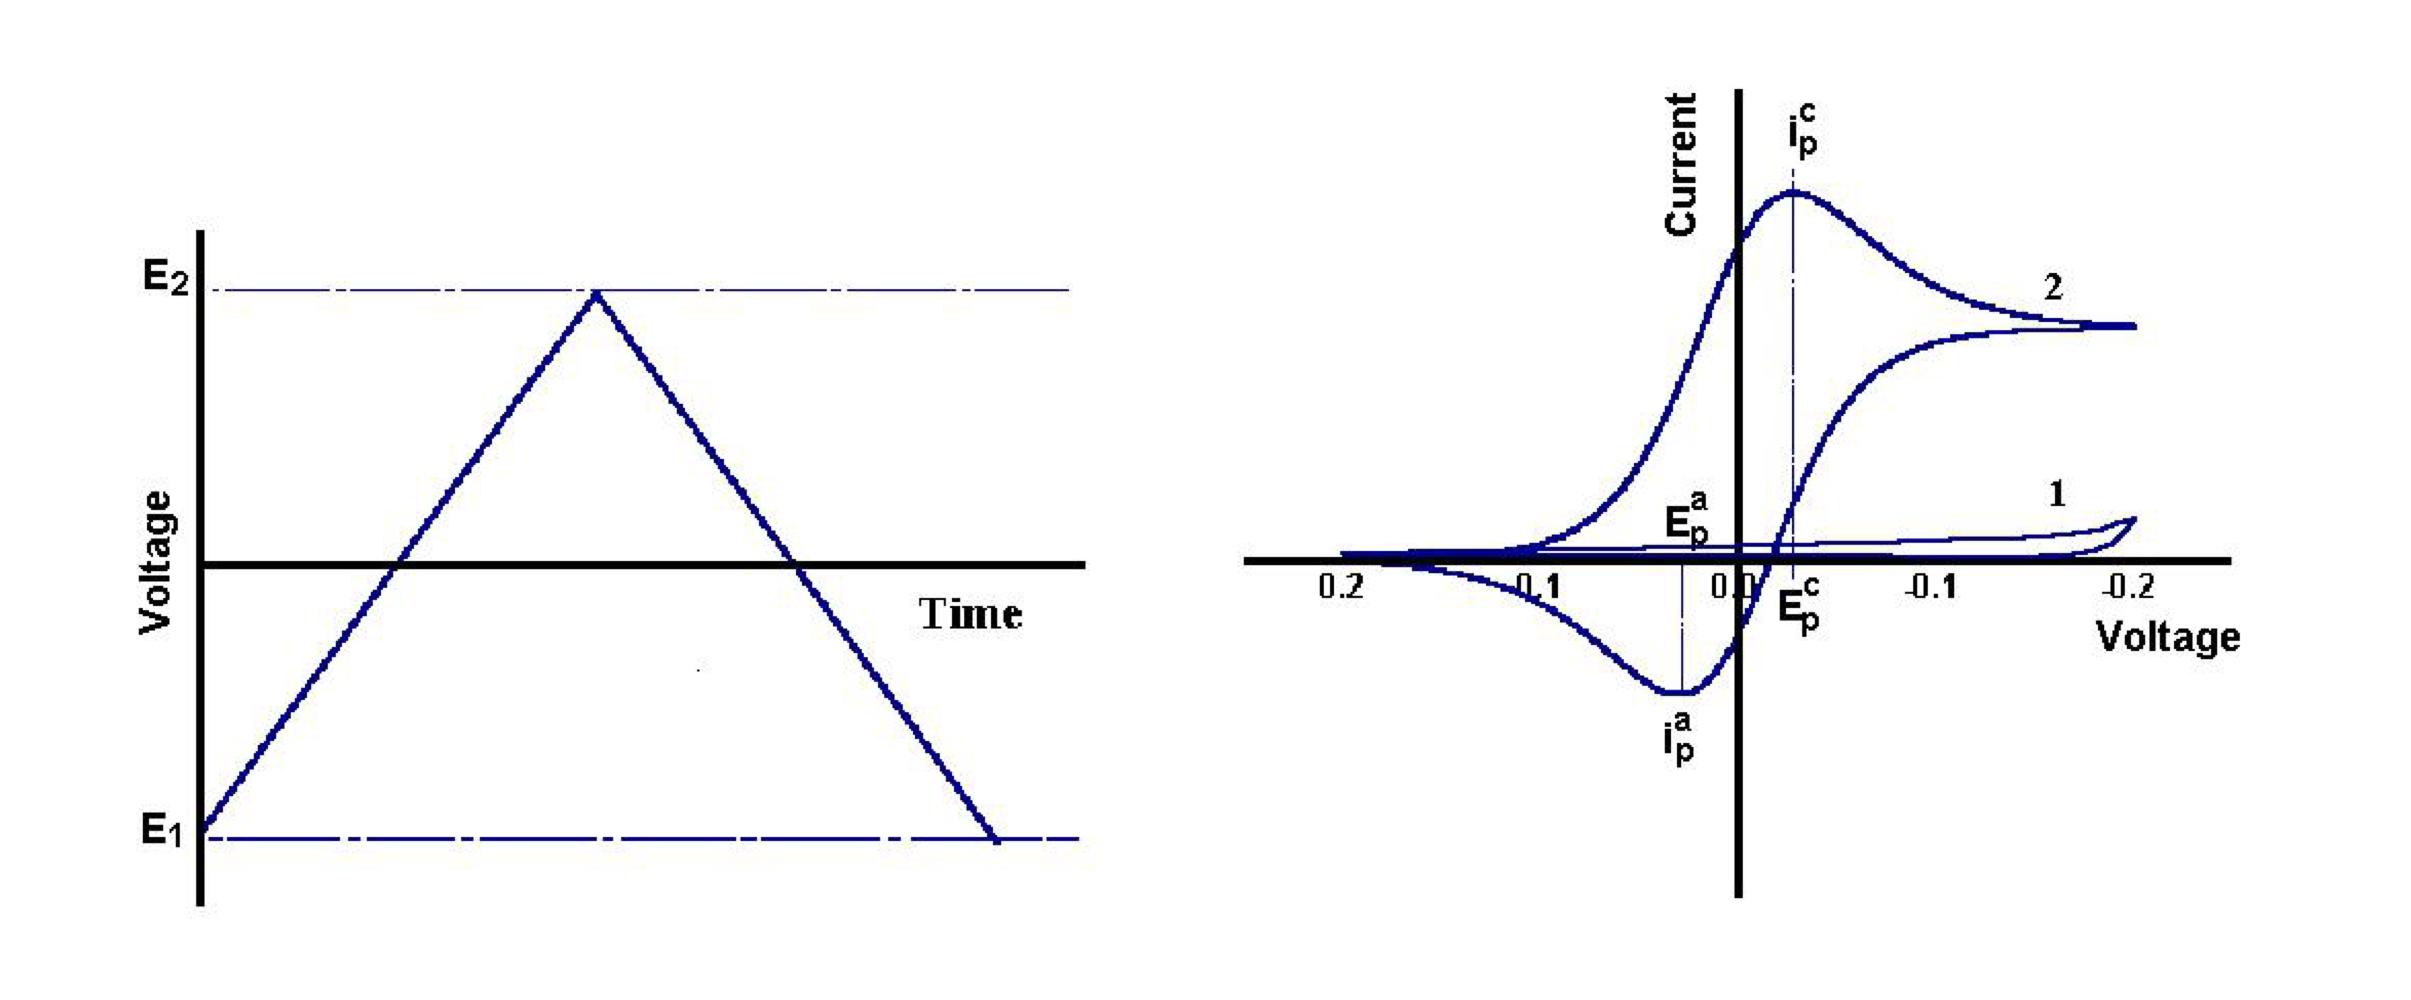
\includegraphics[width=0.7\linewidth]{image/chp7_circular_VA}
%	\caption{}
	\label{fig:chp7circularva}
\end{figure}

\begin{example}
	\begin{figure}[!h]
		\centering
		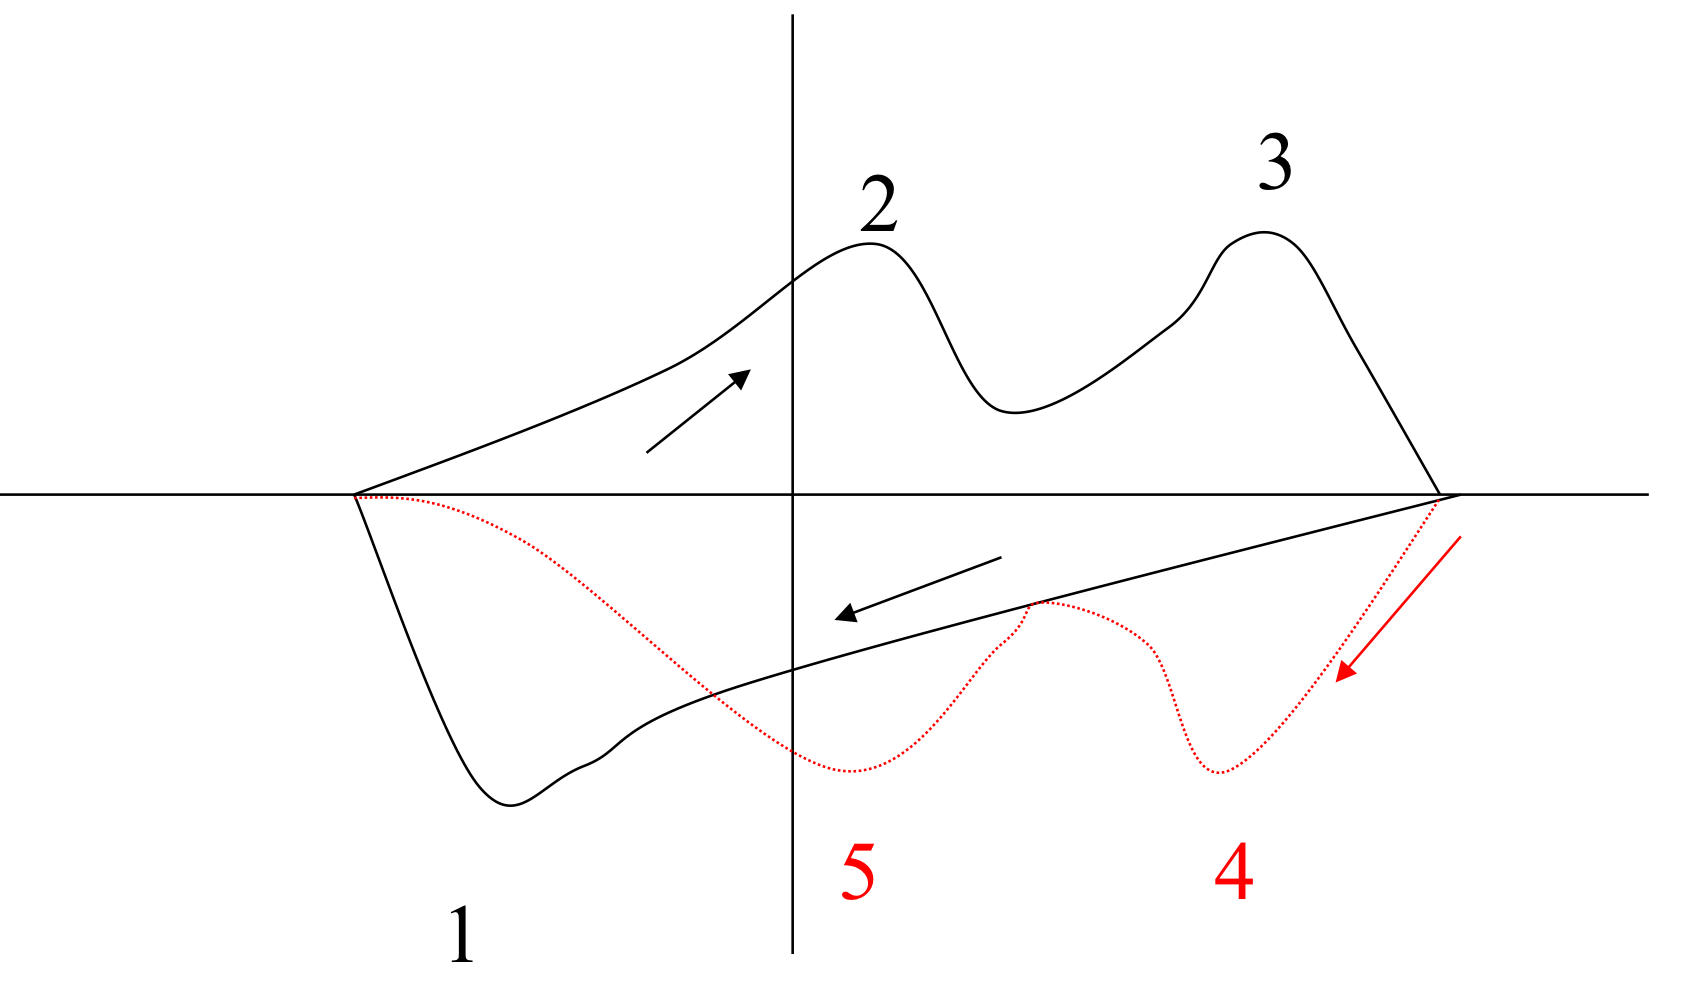
\includegraphics[width=0.7\linewidth]{image/chp7_circular_VA_example}
		\caption{}
		\label{fig:chp7circularvaexample}
	\end{figure}
	图中的几个信号分别对应以下反应:
	\begin{figure}[!h]
		\centering
		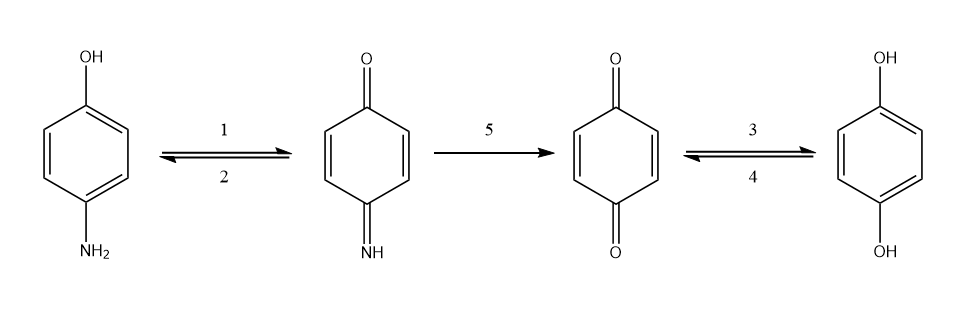
\includegraphics[width=\linewidth]{image/chp7_circular_VA_example_result}
%		\caption{}
		\label{fig:chp7circularvaexampleresult}
	\end{figure}
	
\end{example}

